\chapter{Software Application Architecture}\label{ch:ch2label}
						
						Overall structure of the software application can be represented in the logical grouping of components into layers that interact with each other according to the functionality and features of the application. This chapter will focus on how the application is divided into components and the services provided by each layer.These layers help to uniquely identify the different kind of task performed by each components. Each layer would consist of multiple sub layers which performs specific type of task which would greatly help while debugging.

\begin{figure}[!htb]
  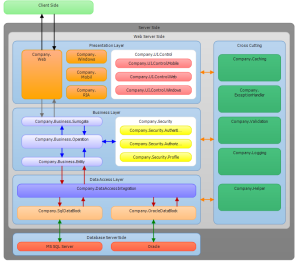
\includegraphics[width=\linewidth]{figures/SwArch.png}
	 \caption{Software Application Architecture}
  \label{fig: Software Application Architecture}
\end{figure}						
					
						By analysing the types of components that exist in most solutions, you can construct a meaningful map of an application or service, and then use this map as a blueprint for your design. Dividing an application into separate layers that have distinct roles and functionalities helps you to maximize maintainability of the code, optimize the way that the application works when deployed in different ways.Figure 2.1 represents the highest and most abstract level of the software architecture.It gives clear perspective of theirs interaction with users, relationship with other application that requests the services implemented within the application business layer,web services hosted by the application , data sources and the remote service used by the applications offered by other software.

\section{Basic Architecture Layer}
						
						The common three layer design consist of Presentation Layer ,Business Layer and Data Layer. 
						
						
\begin{description}
  \item[$\bullet$] {\bfseries Presentation Layer :} This layer consist of two sub components which contains purely user based functionality that manages the user interaction with the application. This layer acts as a bridge between the user and business logic layer. User Interface and user interface logic are the two major components found in this layer.This layer is responsible for the user input and display in addition to the components that organise user Interaction.To make the code modular the implementation of visual elements which would display data to user and accepts input is separated from the presentation logic which gives rise to the idea of model, view and controller.To handle the design based issues , security issues and improve the application performance and user interface responsiveness, the extra components are introduced which discussed in forth coming chapters.
  \item[$\bullet$] {\bfseries Business Layer :} This layer implements core functionality of the application and is concerned with the processing, transformation, retrieval and management of data.The core implementation include the business rules,entities and work flow of the rules. Application façade is a optional component which acts a simplified wrapper on business logic components by combining multiple operations into a single operation in a logical way. This reduces dependencies and improves modularity. This prevents the external service request from knowing the details of the business components and the inter relationship between the operations.
  \item[$\bullet$] {\bfseries Data Layer :} Data access logic and data store are the major components of this layer. Much more components like object document mapper , object relational Mapper etc which deals with translation of data can be introduced into this layer based on the requirements.This layer provides access to data within the boundaries of the system and the data exposed by the other networked systems through web service.Data access logic components forms a interface that the components in the business layer consumes. 
\end{description}			

\section{ Requirement-Based Components  }

			Some layers are pluggable in the architecture on requirement basis.When an application must provide service to external system , the service layer is used to expose the business functionality without exposing the operation signature.There are components which are added to the architecture to handle issues.The issues and the corresponding layer which handles the issue can be categorised based on the architecture layers.
			
\subsection{Issues and Add-on - Presentation Layer}	

\begin{description}
  \item[$\bullet$]{\bfseries Caching :} Caching is considered to be a best mechanism to improve application performance and user interface responsiveness. Caching is used in presentation layer to avoid frequent data lookups which in turn avoids network round trips and to store the result of the repetitive process to avoid the unnecessary duplicated processing. Its important to make the cache thread-safe when it is used in multi-thread environment.
  \item[$\bullet$]{\bfseries Exception Management :} Employing a centralised exception management is considered to be a consistent way to manage the unexpected exceptions. The exception which propagates across layers are blocking issue which would crash the application. Differentiating the error occurred into system-based or business logic based will be helpful to provide a friendly error message to the users. If it is business errors,a error message can be displayed and allow user to re-try that particular operation. In case of system error, a error message can be displayed along with the troubleshooting assistance. It is important to ensure no sensitive data is exposed in the error pages, error message and log files.
  \item[$\bullet$]{\bfseries Compositions :} User interface composition patterns and templates supports the creation of the views and the presentation layout at the run times.It is easy to develop and maintain if the presentation layers uses independent modules and views that are composed at run time. These templates helps to minimise the code and library dependencies that would otherwise force recompilation and redeployment of the modules when the dependencies are upgraded. 
   
\end{description}  		

\subsection{Issues and Add-on - Business Layer}	
  		The business layer includes the previous add-ons like caching 
\begin{description}
  \item[$\bullet$]{\bfseries Caching :} 
\end{description}  

\subsection{Issues and Add-on - Data Layer}	

\begin{description}
  \item[$\bullet$]{\bfseries Caching :} 
\end{description}  

\subsection{Issues and Add-on - Service Layer}	

\begin{description}
  \item[$\bullet$]{\bfseries Caching :} 
\end{description}  